\documentclass{ximera}
\usepackage{sagetex}
%% handout
%% space
%% newpage
%% numbers
%% nooutcomes
 
%% You can put user macros here
%% However, you cannot make new environments

\graphicspath{{./}{module1Activity/}{module2Activity/}{module3Activity/}}

\usepackage{sagetex}
\usepackage{tikz}
\usepackage{hyperref}
\usepackage{tkz-euclide}
\usetkzobj{all}
\pgfplotsset{compat=1.7} % prevents compile error.

\tikzstyle geometryDiagrams=[ultra thick,color=blue!50!black]
 %% we can turn off input when making a master document
 
\outcome{}
\author{Darryl Chamberlain Jr.}
  
\title{Objective 3 - Construct Linear Model}
 
\begin{document}
\begin{abstract}

\end{abstract}

\maketitle
 
% Link to textbook
\href{https://cnx.org/contents/mwjClAV_@15.1:xJt0U6vR@13/2-3-Models-and-Applications}{Construct a model equation for the real-life situation.}
 
%%%%%%%%%%%%%%%%%%%%%
%%%  Objective 3  %%%
%%%%%%%%%%%%%%%%%%%%%

Scenarios we normally use linear functions to model are:
	\begin{itemize}
		\item[\textbf{Finance}] Cost to produce, Utility Bill, Depreciation of Value; 
		\item[\textbf{Motion}] Relative distance of two objects, Using round-trip times to calculate distance, 
		\item[\textbf{Chemistry}] Mixing two different concentrations of solutions;
		\item[\textbf{Statistics}] Line of best fit.
	\end{itemize}

\textbf{After you complete each of the questions below, see if you can put together a ``general form" for the linear model you built.} Here are some videos to help you think about solving linear word problems. \href{https://www.youtube.com/watch?v=ylp6rx1N4P0&list=PLsCqF7qYpC5ZynJm-TTnZ6OsnKOwU7hs_&index=3}{A video to help with some specific problems for this homework can be found here.}

\begin{itemize}
	\item \href{http://openstax.org/l/lineqprobsolve}{Problem solving using linear equations}
	\item \href{http://openstax.org/l/equationprsolve}{Problem solving using equations}
	\item \href{http://openstax.org/l/ratetimesolve}{Distance between two cities}
	\item \href{http://openstax.org/l/lineqappl}{Cost equation word problem} 
\end{itemize}

%%%%%%%%%%%%%%%%%%%%%%%%%
%% Finance Questions %%%%
\begin{sagesilent}
x = var("x")
fixedCost1 = ZZ.random_element(10, 26)*1000
productionCost1 = round(ZZ.random_element(1, 4)*0.05, 2)
sellingPoint1 = round(productionCost1*ZZ.random_element(1, 4), 2)
costs1 = productionCost1*x + fixedCost1
profits1 = sellingPoint1*x
revenue1 = profits1 - costs1
\end{sagesilent}

\begin{exercise}
A company sells doughnuts. They incur a fixed cost of \$$\sage{fixedCost1}$ for rent, insurance, and other expenses. It costs \$$\sage{productionCost1}$ to produce each doughnut. The company sells each doughnut for \$$\sage{sellingPoint1}$.

\textbf{Part A.} Construct a linear model that describes their total costs, $C$, as a function of the number of doughnuts, $x$, they produce.

$C(x) = \answer{\sage{costs1}}$

\textbf{Part B.} Construct a linear model that describes their total profits, $P$, as a function of the number of doughnuts, $x$, they produce.

$P(x) = \answer{\sage{profits1}}$

\textbf{Part C.} Construct a linear model that describes their total revenue, $R$, as a function of the number of doughnuts, $x$, they produce.

$R(x) = \answer{\sage{revenue1}}$

\end{exercise}

\begin{sagesilent}
x = var('x')
savings2 = ZZ.random_element(5, 11)*1000
rent2 = ZZ.random_element(7, 12)*100
food2 = ZZ.random_element(4, 8)*10
misc2 = ZZ.random_element(4, 8)*8
costs2 = (rent2 + 4*food2 + 4*misc2)*x
profits2 = 300 + savings2
revenue2 = profits2 - costs2
\end{sagesilent}

\begin{exercise}
Aubrey is a college student going into her first year at UF. She will receive Bright Futures, which covers her tuition plus a \$300 educational expense each Fall and Spring semester. Before college, Aubrey saved up $\$\sage{savings2}$. She knows she will need to pay $\$\sage{rent2}$ in rent a month, $\$\sage{food2}$ for food a week, and $\$\sage{misc2}$ in other weekly expenses.

\textbf{Part A.} Construct a linear model that describes her total costs, $C$ as a function of the number of months, $x$, she is at UF \textbf{during Fall semester}. 

$C(x) = \answer{\sage{costs2}}$

\textbf{Part B.} Construct a linear model that describes her total income, $I$, as a function of the number of months, $x$, she is at UF \textbf{during Fall semester}.

$I(x) = \answer{\sage{profits2}}$

\textbf{Part C.} Construct a linear model that describes their total budget, $B$, as a function of the number of months, $x$, she is at UF \textbf{during Fall semester}.

$B(x) = \answer{\sage{revenue2}}$
\end{exercise}

\textbf{\Large Try to write down notes on how to solve the first two questions \textit{in general}.}

%%%%%%%%%%%%%%%%%%%%%%%%%
%% Motion Questions %%%%%
\begin{sagesilent}
m = var('m')
officerAspeed3 = ZZ.random_element(2, 5)
officerBspeed3 = ZZ.random_element(2, 5)
partA3 = officerAspeed3/60 * m
partB3 = officerAspeed3/60 * m + officerBspeed3/60 * m
partC3 = sqrt((officerAspeed3/60)**2 + (officerBspeed3/60)**2)*m
\end{sagesilent}

\begin{exercise}
Two UFPD are patrolling the campus on foot. To cover more ground, they split up and begin walking in different directions. Office A is walking at $\sage{officerAspeed3}$ mph while Office B is walking at $\sage{officerBspeed3}$ mph. 

\textbf{Part A.} Construct a linear model that describes Officer A's distance from their starting point, $D$, as a function of minutes, $m$, that have passed.

$D(m) = \answer{\sage{partA3}}$

\begin{hint}
	$\text{Speed} = \frac{\text{distance}}{\text{time}}$
	
	Can you re-solve this for distance?
\end{hint}

\textbf{Part B.} Construct a linear model that describes their total distance from each other, $T_1$, as a function of minutes, $m$, that have passed \textit{if they were walking in exactly opposite directions} (e.g., North/South).

$T_1(m) = \answer{\sage{partB3}}$

\textbf{Part C.} Construct a linear model that describes their total distance from each other, $T_2$, as a function of minutes, $m$, that have passed \textit{if they were walking in exactly 90 degrees from each other} (e.g., North/East).

$T_2(m) = \answer{\sage{partC3}}$

\textit{Exact value needed for the coefficient! DO NOT ROUND.}

\begin{hint}
For Part C, draw a picture and think about how the Pythagorean Theorem could be used. Remember: these are all linear models! So if your model has a non-linear \textbf{variable}, is there a reason we would ignore part of the domain?
\end{hint}
\end{exercise}

% Bike question
\begin{sagesilent}
t, D = var('t', 'D')
speedFlat4 = ZZ.random_element(3, 6)
speedUp4 = speedFlat4 - ZZ.random_element(1, 3)
speedDown4 = speedFlat4 + ZZ.random_element(2, 4)
partC4 = (speedFlat4 + speedUp4 + speedDown4)*t
partD4 = D*(1/speedUp4 + 1/speedDown4 + 1/speedFlat4)
\end{sagesilent}

\begin{exercise}
\begin{figure}
	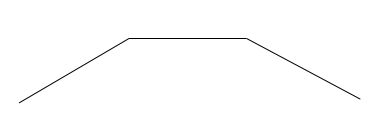
\includegraphics[scale=0.5]{pathHW.png}
	\caption{Training path.}
\end{figure}
A bicyclist is training for a race on a hilly path. Their bike keeps track of their speed at any time, but not the distance traveled. Their speed traveling up a hill is $\sage{speedUp4}$mph, $\sage{speedDown4}$mph when traveling down a hill, and $\sage{speedFlat4}$mph when traveling along a flat portion. 

\begin{hint}
Distance is equal to rate times time. 
\end{hint}

\textbf{Part A.} Construct linear models that describe their distance, $D$ in miles, on a particular portion of the path in terms of the time, $t$ in hours, spent on that part of the path. 

$D_{\text{up}}(t) = \answer{\sage{speedUp4*t}}$

$D_{\text{down}}(t) = \answer{\sage{speedDown4*t}}$

$D_{\text{flat}}(t) = \answer{\sage{speedFlat4*t}}$

\textbf{Part B.} Construct linear models that describe their time, $t$ in hours, on a particular portion of the path in terms of the length, $D$ in miles, of that part of the path.

$t_{\text{up}}(D) = \answer{\sage{D/speedUp4}}$ 

$t_{\text{down}}(D) = \answer{\sage{D/speedDown4}}$

$t_{\text{flat}}(D) = \answer{\sage{D/speedFlat4}}$

\textbf{Part C.} Construct a linear model that describes the total distance of the path, $D$, in terms of the time spent on a particular path \textit{if we knew that the time spent on each path was equal}.

$D(t) = \answer{\sage{partC4}}$

\textbf{Part D.} Construct a linear model that describes the total time $T$ spent on the path in terms of the distance of a particular part of the path \textit{if we knew that all parts of the path are equal length}.

$T(D) = \answer{\sage{partD4}}$

\end{exercise}

%%%%%%%%%%%%%%%%%%%%%%%%%
%% "Mixture" Questions %%
\begin{sagesilent}
x = var('x')
teenTicketPrice = ZZ.random_element(3, 7)
adultTicketPrice = teenTicketPrice + ZZ.random_element(3, 7)
teenTicketCount = ZZ.random_element(30, 70)
adultTicketCount = ZZ.random_element(30, 70)
totalTickets = teenTicketCount + adultTicketCount
totalRevenue = teenTicketCount*teenTicketPrice + adultTicketCount*adultTicketPrice
eqPartA5 = totalTickets - x
eqPartB5 = eqPartA5 * adultTicketPrice
eqPartC5 = eqPartB5 + teenTicketPrice * x
\end{sagesilent}

\begin{exercise}
Kappa Delta is hosting an all-you-can-eat pancake fundraiser to support the prevention of child abuse. Adult (18+) tickets are $\$ \sage{adultTicketPrice}$ and teen (10-17) tickets are $\$\sage{teenTicketPrice} $. Children under 10 are let in without a ticket. The ticket-sellers only kept track of the total number of tickets sold, $\sage{totalTickets}$, and total revenue, $\$ \sage{totalRevenue}$. 

\textbf{Part A.} Construct a linear model that describes the total number of adult tickets, $y$, sold in terms of the number of teen tickets, $x$, sold.

$y = \answer{\sage{eqPartA5}}$

\textbf{Part B.} Construct a linear model that describes the revenue made from selling many adult tickets, $R_a$, in terms of the number of teen tickets, $x$, sold. 

$R_a = \answer{\sage{eqPartB5}}$

\textbf{Part C.} Construct a linear model that describes the total revenue made, $R_T$, in terms of the number of teen tickets, $x$, sold. 

$R_T = \answer{\sage{eqPartC5}}$

\begin{hint}
Part A: Is there way to build an equation that relates adult tickets, teen tickets, and total tickets? Solving this equation for adult tickets would give you the linear model.

Part B: It may be easier to first build this model in terms of $y$, then use your answer from part A.

Part C: Think about how to model total revenue, then use your answer in Part B to make part of the model.
\end{hint}
\end{exercise}

\begin{sagesilent}
v = var('v')
concA = ZZ.random_element(1, 4)*5
concB = ZZ.random_element(2, 5)*10
concTotal = ZZ.random_element(10, 31)
while concTotal < concA or concTotal > concB:
    concTotal = ZZ.random_element(10, 31)
totalVolume = ZZ.random_element(5, 15)
eqPartA6 = totalVolume - v
eqPartB6 = concA * 0.01 * v
eqPartC6 = concB * 0.01 * eqPartA6
eqPartD6 = eqPartB6 + eqPartC6
\end{sagesilent}
\begin{exercise}
Chemists commonly create a solution by mixing two products of differing concentrations together. For example, a chemist could have large amounts of a $\sage{concA}\%$ acid solution and a $\sage{concB}\%$ acid solution, but need a $\sage{totalVolume}$ liter $\sage{concTotal}$\% solution.

\textbf{Part A.} Construct a linear model that describes the volume of the $\sage{concB}\%$ acid solution, $v_{\sage{concB}}$, in terms of the volume of the $\sage{concA}\%$ acid solution, $v$. 

$v_{\sage{concB}} = \answer{\sage{eqPartA6}}$

\textbf{Part B.} Construct a linear model that describes the amount of acid in a $\sage{concA}\%$ acid solution, $A_{\sage{concA}}$, in terms of the volume of the $\sage{concA}\%$ acid solution, $v$. 

$A_{\sage{concA}} = \answer{\sage{eqPartB6}} $

\textbf{Part C.} Construct a linear model that describes the amount of acid in a $\sage{concB}\%$ acid solution, $A_{\sage{concB}}$, in terms of the volume of the $\sage{concA}\%$ acid solution, $v$. 

$A_{\sage{concB}} = \answer{\sage{eqPartC6}} $

\textbf{Part D.} Construct a linear model that describes the amount of acid in a $\sage{concTotal}\%$ acid solution, $A_{\sage{concTotal}}$, in terms of the volume of the $\sage{concA}\%$ acid solution, $v$. 

$A_{\sage{concTotal}} = \answer{\sage{eqPartD6}}$

\begin{hint}
Parts A-D: Think about what you did in the last problem. How can we use that same structure in this new setting?
\end{hint}

\end{exercise}

\end{document}